\chapter{Feuille XSLT pour transformer les exports SKOS en CSV} \label{skos2csv}

\begin{codeblock}{xslt}
<?xml version="1.0" encoding="UTF-8"?>
<xsl:stylesheet version="2.0"
    xmlns:xsl="http://www.w3.org/1999/XSL/Transform"
    xmlns:skos="http://www.w3.org/2004/02/skos/core#"
    xmlns:rdf="http://www.w3.org/1999/02/22-rdf-syntax-ns#"
    exclude-result-prefixes="skos rdf">

    <xsl:output method="text" encoding="UTF-8"/>

    <!-- Header -->
    <xsl:template match="/">
        <xsl:text>URI;skos:prefLabel;skos:altLabel;skos:narrower;skos:broader;skos:scopeNote&#10;</xsl:text>
        <xsl:apply-templates select="//skos:Concept"/>
    </xsl:template>

    <!-- Concept rows -->
    <xsl:template match="skos:Concept">
        <!-- URI -->
        <xsl:value-of select="@rdf:about"/>
        <xsl:text>;</xsl:text>

        <!-- prefLabel -->
        <xsl:value-of select="normalize-space(skos:prefLabel[@xml:lang='fr'])"/>
        <xsl:text>;</xsl:text>

        <!-- altLabel(s) -->
        <xsl:for-each select="skos:altLabel[@xml:lang='fr']">
            <xsl:value-of select="normalize-space(.)"/>
            <xsl:if test="position() != last()">,</xsl:if>
        </xsl:for-each>
        <xsl:text>;</xsl:text>

        <!-- narrower(s) -->
        <xsl:for-each select="skos:narrower">
            <xsl:value-of select="@rdf:resource"/>
            <xsl:if test="position() != last()">,</xsl:if>
        </xsl:for-each>
        <xsl:text>;</xsl:text>

        <!-- broader(s) -->
        <xsl:for-each select="skos:broader">
            <xsl:value-of select="@rdf:resource"/>
            <xsl:if test="position() != last()">,</xsl:if>
        </xsl:for-each>
        <xsl:text>;</xsl:text>

        <!-- scopeNote -->
        <xsl:value-of select="normalize-space(skos:scopeNote[@xml:lang='fr'])"/>
        <xsl:text>&#10;</xsl:text>
    </xsl:template>

</xsl:stylesheet>
\end{codeblock}

\chapter{Philidor Scraper : Outil de collecte et de téléchargement des ressources du catalogue Philidor}  \label{philidor_scrapper}

\section*{Introduction}

Cette annexe présente le livrable \textbf{Philidor Scraper}, un outil développé dans le cadre de ce mémoire pour automatiser la collecte et le téléchargement des documents du catalogue de notice bibliographique Philidor, mis en ligne par le Centre de Musique Baroque de Versailles. 

Le code source est librement accessible sur GitHub à l'adresse suivante : 
\url{https://github.com/AmelieDogan/Philidor_scraper}. 

Cet outil répond au besoin de recenser et de sauvegarder des documents (partitions, manuscrits, etc.) associés aux notices présentes dans la base Philidor en vu de la migration des notices d'\textit{eZ Publish} vers PMB. 
Il permet à la fois de générer un fichier récapitulatif des ressources disponibles et de télécharger automatiquement les documents correspondants, en assurant une organisation claire et normalisée des fichiers.

\section*{Architecture et fonctionnement}
Le \textit{Philidor Scraper} est conçu comme un script Python unique, \texttt{philidor\_scraper.py}, organisé autour d'une classe principale \texttt{PhilidorScraper}.  
Le processus global se décompose en plusieurs étapes successives :

\begin{enumerate}
    \item \textbf{Initialisation et configuration} :  
    Le script configure une session HTTP et crée un dossier local (\texttt{philidor\_documents/}) pour stocker les fichiers téléchargés.  
    Une gestion des logs est mise en place dans le fichier \texttt{philidor\_scraper.log} pour suivre l'exécution et détecter d'éventuelles erreurs.

    \item \textbf{Scraping du catalogue} :  
    Le scraper parcourt les pages du catalogue en incrémentant un \texttt{offset} et récupère les \textbf{numéros de notice} ainsi que les \textbf{liens directs} vers les documents disponibles.  
    Ces informations sont stockées dans une structure Python avant d'être exportées dans un fichier CSV (\texttt{philidor\_results.csv}).

    \item \textbf{Normalisation des noms de fichiers} :  
    Les fichiers récupérés peuvent contenir des accents, espaces ou caractères spéciaux.  
    Une fonction dédiée génère des noms de fichiers propres et standardisés, intégrant le numéro de notice pour faciliter le classement.

    \item \textbf{Téléchargement automatique} :  
    Une fois la phase de scraping terminée, l'utilisateur peut choisir de télécharger tous les fichiers trouvés.  
    Des pauses automatiques sont intégrées pour ne pas surcharger le serveur.

    \item \textbf{Export des résultats} :  
    L'ensemble des données collectées (identifiants, liens, fichiers) est exporté dans un fichier \texttt{philidor\_results.csv}.  
    Ce fichier peut être exploité pour des traitements ultérieurs ou pour des analyses statistiques.
\end{enumerate}

\section*{Avantages et apports du scraper}
Le \textit{Philidor Scraper} présente plusieurs atouts dans le contexte de ce projet :

\begin{itemize}
    \item \textbf{Automatisation complète} : le script supprime la nécessité de télécharger manuellement chaque document depuis le site.
    \item \textbf{Fiabilité des données} : grâce à la normalisation des noms de fichiers et à l'utilisation d'identifiants uniques, l'organisation des fichiers est claire et cohérente.
    \item \textbf{Respect du serveur} : l'intégration de pauses automatiques limite l'impact sur les performances du site Philidor.
    \item \textbf{Traçabilité} : le fichier CSV et les logs permettent de suivre précisément les documents collectés et téléchargés.
\end{itemize}

\section*{Conclusion}

Le \textit{Philidor Scraper} a constitué un outil pratique et efficace pour collecter et sauvegarder en masse les ressources du catalogue Philidor.  
Il automatise un processus long et fastidieux tout en assurant une organisation claire et traçable des données.

\chapter{Le pipeline de hiérarchisation semi-automatique du thésaurus}
\label{pipeline-hierarchisation-theso}

\section*{Introduction}

Cette annexe présente le prototype de pipeline \textbf{Thesaurus Hierarchizer} développé dans le cadre de ce mémoire, dont l'objectif est d'assister à la hiérarchisation d'un thésaurus musical.

Le code source est accessible sur la plateforme GitHub à l'adresse suivante : \url{https://github.com/AmelieDogan/thesaurus-hierarchizer.git}.

Ce pipeline vise à enrichir un thésaurus en identifiant et en ajoutant des relations hiérarchiques de type \codeinline{text}{skos:broader} et \codeinline{text}{skos:narrower} de manière semi-automatique, réduisant ainsi le travail manuel fastidieux.

\section*{Architecture et Phases du Pipeline}

L'architecture du pipeline est conçue de manière modulaire, chaque phase étant gérée par un script Python dédié. Cette approche permet de suivre le processus de hiérarchisation étape par étape et de faciliter la maintenance ou l'ajout de nouvelles fonctionnalités. L'ensemble du processus est orchestré par le script principal \texttt{main\_orchestrator.py}. Le pipeline se décompose comme suit :

\begin{enumerate}
	\item \textbf{phase1\_data\_processor.py} : Prétraitement des données. Le pipeline prend en entrée un fichier au format \gls{csv} avec le séparateur tabulation qui contient des concepts déjà structurés au format SKOS mais sans URI. Il génère donc les URIs pour chaque concept. Une des forces de cette phase réside dans sa capacité à vérifier et à enrichir les relations parentales existantes. Si un concept est désigné comme parent potentiel par son \texttt{prefLabel} (et non par son URI), le pipeline recherche si ce label existe déjà dans le thésaurus. S'il est trouvé, le lien est remplacé par son URI, garantissant la cohérence des données. Dans le cas contraire, une intervention de l'utilisateur sera requise à la phase 5 pour valider la création du nouveau concept et de son URI.
	
	\item \textbf{phase2\_pattern\_detector.py} : Détection par inclusion lexicale. Cette phase identifie des relations hiérarchiques en se basant sur des patterns d'inclusion de termes. Par exemple, elle reconnaît automatiquement que le concept \textquote{flûte à bec} est plus spécifique que \textquote{flûte}. Ces liens sont considérés comme très fiables et sont automatiquement ajoutés à la hiérarchie.
	
	\item \textbf{phase3\_similarity\_analyzer.py} : Analyse de la similarité lexicale. En explorant les familles lexicales, cette phase propose des liens de parenté en choisissant le terme le plus court comme parent potentiel (par exemple, \textquote{liturgie} pour \textquote{liturgique}). L'approche pourrait nécessiter des ajustements précis, notamment au niveau de sa configuration via le fichier \codeinline{text}{config.py} pour optimiser les résultats.
	
	\item \textbf{phase4\_contextual\_embedding\_analyzer.py} : Détection par similarité vectorielle. Cette phase tire parti de modèles de \textit{word embeddings} (ici camemBERT) pour analyser les similarités sémantiques entre les concepts. Les concepts sont regroupés en clusters, et le pipeline propose un terme qui semble le mieux représenter ce groupe. L'utilisateur peut ensuite valider, rejeter ou modifier ce terme pour enrichir la hiérarchie de manière sémantiquement pertinente.
	
	\item \textbf{phase5\_hierarchy\_builder.py} : Construction de la hiérarchie finale et validation de tous les parents candidats pour des groupes de concepts par l'utilisateur.
	
	\item \textbf{phase6\_hierarchy\_optimizer.py} : Optimisation de la hiérarchie.
	
	\item \textbf{phase7\_output\_generator.py} : Génération des livrables finaux, incluant un thésaurus enrichi sous deux formats et un rapport HTML détaillé.

\end{enumerate}

\section*{Avantages du Pipeline}

Le développement de ce prototype offre plusieurs avantages significatifs :

\begin{itemize}
	\item \textbf{Efficacité du traitement de données} : La prise en charge directe d'un fichier CSV (séparateur tabulation) facilite l'intégration dans un flux de travail de gestion de données existant.
	\item \textbf{Validation et enrichissement automatique} : Le pipeline gère intelligemment la conversion des \texttt{prefLabel} en URI, réduisant les incohérences et les erreurs de saisie.
	\item \textbf{Diversité des méthodes d'analyse} : La combinaison de patterns lexicaux, de l'analyse de similarité et des embeddings sémantiques garantit une détection de relations à la fois précise et variée.
	\item \textbf{Approche semi-automatique} : L'implication de l'utilisateur pour la validation des relations et la création de nouveaux concepts permet de maintenir la qualité et la pertinence du thésaurus.
\end{itemize}

\section*{Perspectives et Axes d'Amélioration}

Bien que le prototype soit fonctionnel et efficace, plusieurs pistes d'amélioration pourraient enrichir ses capacités :

\begin{itemize}
	\item \textbf{Meilleure gestion des relations existantes} : Le pipeline prend en entrée des relations écrites sous la forme de \codeinline{text}{prefLabel} qui pourrait être parent. Il serait pertinent de prendre également en charge des relations déjà référencées par des URIs et de permettre une validation manuelle précoce des relations candidates dès cette phase, plutôt qu'en phase 5. Cela enrichirait le contexte pour l'analyse par \textit{embeddings}.
	\item \textbf{Interopérabilité avec des thésaurus externes} : L'ajout d'une fonctionnalité permettant d'utiliser des thésaurus externes comme sources de données supplémentaires aiderait le pipeline à trouver davantage de relations (par exemple, \codeinline{text}{skos:closeMatch} ou \codeinline{text}{skos:exactMatch}).
	\item \textbf{Validation granulaire des groupes} : Pour les groupes de concepts dont le parents est à valider manuellement, il serait pertinent de permettre à l'utilisateur de valider individuellement les termes, notamment si le groupe contient des intrus ou s'il est composé de plusieurs sous-groupes plus petits.
	\item \textbf{Détection de doublons} : Une étape supplémentaire pourrait être ajoutée en fin de processus pour détecter d'éventuels doublons de concepts. Cela permettrait de repérer les concepts malencontreusement ajoutés en double, renforçant ainsi la cohérence du thésaurus.
\end{itemize}

\section*{Conclusion}

Le pipeline de hiérarchisation semi-automatique représente un outil puissant pour la gestion et l'enrichissement des thésaurus. Il automatise les tâches fastidieuses tout en préservant le contrôle humain sur les décisions finales. Les axes d'amélioration identifiés ouvrent la voie à une version plus robuste et interactive, capable de s'adapter à des cas d'usage plus complexes.

\chapter{L'application XML to WEB App pour l'édition web statique Philidor Vitrine} 
\label{xml_to_web_app}

\section*{Introduction}

Cette annexe présente le livrable \textbf{XML to WEB App}, une application développée dans le cadre de ce mémoire pour faciliter la publication en ligne des données issues de \textit{Philidor 4} sous forme d'une édition web statique, nommée \textit{Philidor Vitrine}.  

Le code source de l'application est accessible sur GitHub à l'adresse suivante :  
\url{https://github.com/AmelieDogan/philidorvitrine.git}.

L'objectif principal de cette application est d'automatiser la transformation de données complexes au format XML, représentant les notices de la base de données \textit{Philidor 4}, en un site web statique complet et consultable. Cette automatisation réduit considérablement la charge de travail liée à la création et à la maintenance de l'édition numérique, tout en garantissant une cohérence et une accessibilité optimales pour les utilisateurs finaux.

\section*{Architecture et fonctionnement}

L'architecture de l'application repose sur une séparation claire entre les différents composants : 

\begin{itemize}
    \item \textbf{Données XML} : elles contiennent le contenu brut des notices et les informations éditoriales des projets issus de \textit{Philidor 4} et de l'édition numérique elle-même.
    \item \textbf{Transformations XSLT} : elles définissent la logique de génération des pages web à partir des données XML grâce à la feuille XSLT et au moteur de transformation.
    \item \textbf{Feuilles de style CSS et autres éléments de mise en page} : elles contrôlent l'apparence et la mise en page des pages générées.
    \item \textbf{Interface utilisateur} : elle offre un environnement visuel pour paramétrer et lancer la transformation sans nécessiter de manipulations techniques.
\end{itemize}

Le processus global suit les étapes suivantes :

\begin{enumerate}
    \item Configuration du contenu de présentation de l'édition numérique et des pages légales via les éditeurs WYSIWYG.
    \item Ajout des projets et de leurs éléments descriptifs (titre, identifiants \textit{Philidor 4} et description).
    \item Importation du panier de données XML extrait de \textit{Philidor 4}
    \item Lancement de la transformation XSLT et téléchargement du site web.
\end{enumerate}

\section*{Avantages de l'application XML to WEB App}

Le développement de cette application offre plusieurs avantages significatifs pour la gestion et la diffusion des éditions numériques de \textit{Philidor 4} :

\begin{itemize}
    \item \textbf{Efficacité de la publication} :  
    L'application automatise la transformation de données XML complexes en un site web statique complet, incluant l'index, les mentions légales et toutes les pages de projets.  
    Cela réduit considérablement le temps et les efforts nécessaires pour publier l'édition numérique \textit{Philidor Vitrine}.

    \item \textbf{Contrôle et gestion simplifiée} :  
    Grâce à une interface graphique intuitive, les utilisateurs peuvent modifier le contenu éditorial sans avoir à manipuler directement les fichiers XML ou les transformations XSLT, garantissant ainsi la cohérence et la fiabilité des données.

    \item \textbf{Séparation claire des responsabilités} :  
    La séparation des données (XML), de la logique de transformation (XSLT) et du design (CSS) facilite la maintenance et l'évolution de chaque composant indépendamment.

    \item \textbf{Accessibilité et documentation} :  
    L'application inclut une page d'accueil avec des conseils d'utilisation et un onglet d'aide complet, ce qui la rend accessible même à des utilisateurs non techniques et réduit la courbe d'apprentissage.
\end{itemize}

\section*{Perspectives et axes d'amélioration}

Bien que l'application soit déjà un outil fonctionnel et efficace, plusieurs pistes d'amélioration peuvent être envisagées pour enrichir ses fonctionnalités et la rendre encore plus robuste :

\begin{itemize}
    \item \textbf{Mise à jour automatique des dépendances} :  
    Mise en place d'un système qui vérifie et notifie l'utilisateur des mises à jour des dépendances XML et XSLT utilisées par l'édition numérique, afin d'assurer la compatibilité et la sécurité du projet.

    \item \textbf{Prévisualisation en temps réel} :  
    Ajout d'une fonctionnalité permettant de prévisualiser les pages web générées directement dans l'application avant la transformation finale, afin de vérifier instantanément les modifications.

    \item \textbf{Gestion des versions de projets} :  
    Intégration d'un système simple de gestion des versions pour les projets, avec un historique des sauvegardes, permettant de restaurer des versions antérieures en cas d'erreur.

    \item \textbf{Surveillance de la connexion internet} :  
    Intégration d'un mécanisme pour vérifier la disponibilité du réseau, indispensable au bon fonctionnement de l'éditeur qui nécessite une connexion active.
\end{itemize}

\section*{Conclusion}

L'application \textit{XML to WEB App} constitue un outil clé pour la publication d'éditions numériques complexes à partir de données XML, telles que celles du projet \textit{Philidor Vitrine}.  
Elle simplifie et accélère le processus de génération de sites web statiques tout en maintenant une séparation claire entre données, transformations et design.

\chapter{Philidor 4 - Contenu et recherche} \label{philidor4-contenu-recherche}

% Première page sous le titre
\begin{center}
	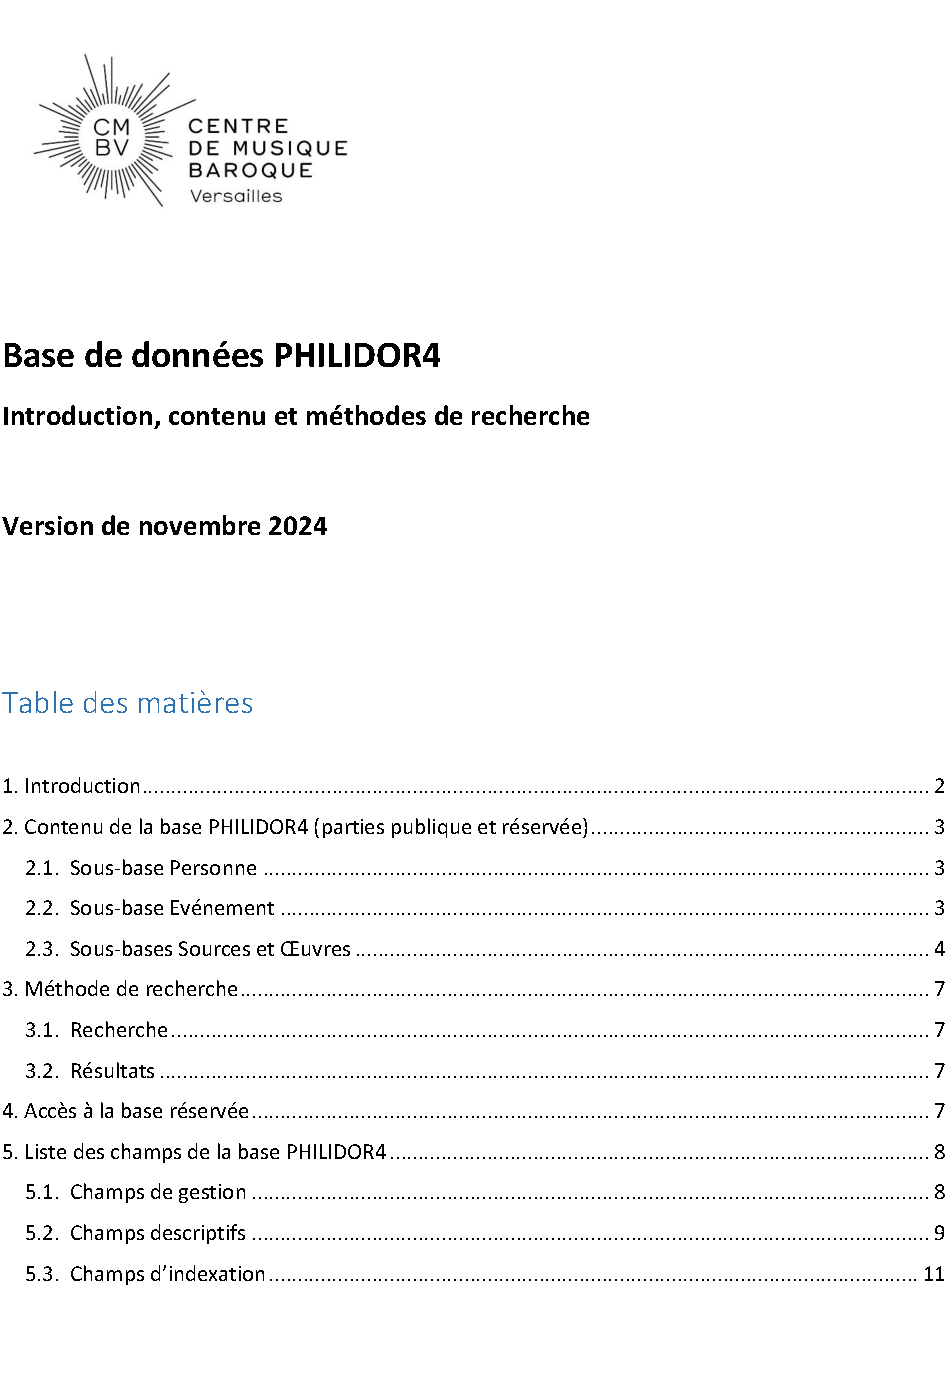
\includegraphics[page=1,width=0.7\textwidth,keepaspectratio]{pdf/PHILIDOR4 - Contenu et recherche cropped.pdf}
\end{center}

% Les pages suivantes, centrées aussi
\foreach \p in {2,...,11}{%
	\clearpage
	\begin{center}
		\includegraphics[page=\p,width=0.7\textwidth,keepaspectratio]{pdf/PHILIDOR4 - Contenu et recherche cropped.pdf}
	\end{center}
}